% Options for packages loaded elsewhere
\PassOptionsToPackage{unicode}{hyperref}
\PassOptionsToPackage{hyphens}{url}
\documentclass[
  10pt,
  a4paper,
]{article}
\usepackage{xcolor}
\usepackage[margin=22mm]{geometry}
\usepackage{amsmath,amssymb}
\setcounter{secnumdepth}{-\maxdimen} % remove section numbering
\usepackage{iftex}
\ifPDFTeX
  \usepackage[T1]{fontenc}
  \usepackage[utf8]{inputenc}
  \usepackage{textcomp} % provide euro and other symbols
\else % if luatex or xetex
  \usepackage{unicode-math} % this also loads fontspec
  \defaultfontfeatures{Scale=MatchLowercase}
  \defaultfontfeatures[\rmfamily]{Ligatures=TeX,Scale=1}
\fi
\usepackage{lmodern}
\ifPDFTeX\else
  % xetex/luatex font selection
\fi
% Use upquote if available, for straight quotes in verbatim environments
\IfFileExists{upquote.sty}{\usepackage{upquote}}{}
\IfFileExists{microtype.sty}{% use microtype if available
  \usepackage[]{microtype}
  \UseMicrotypeSet[protrusion]{basicmath} % disable protrusion for tt fonts
}{}
\makeatletter
\@ifundefined{KOMAClassName}{% if non-KOMA class
  \IfFileExists{parskip.sty}{%
    \usepackage{parskip}
  }{% else
    \setlength{\parindent}{0pt}
    \setlength{\parskip}{6pt plus 2pt minus 1pt}}
}{% if KOMA class
  \KOMAoptions{parskip=half}}
\makeatother
\usepackage{graphicx}
\makeatletter
\newsavebox\pandoc@box
\newcommand*\pandocbounded[1]{% scales image to fit in text height/width
  \sbox\pandoc@box{#1}%
  \Gscale@div\@tempa{\textheight}{\dimexpr\ht\pandoc@box+\dp\pandoc@box\relax}%
  \Gscale@div\@tempb{\linewidth}{\wd\pandoc@box}%
  \ifdim\@tempb\p@<\@tempa\p@\let\@tempa\@tempb\fi% select the smaller of both
  \ifdim\@tempa\p@<\p@\scalebox{\@tempa}{\usebox\pandoc@box}%
  \else\usebox{\pandoc@box}%
  \fi%
}
% Set default figure placement to htbp
\def\fps@figure{htbp}
\makeatother
\setlength{\emergencystretch}{3em} % prevent overfull lines
\providecommand{\tightlist}{%
  \setlength{\itemsep}{0pt}\setlength{\parskip}{0pt}}
\usepackage{mathrsfs}
\usepackage{mathtools}
\usepackage{xurl}
\emergencystretch=3em
\setcounter{tocdepth}{1}
\newcommand{\Beta}{\mathrm{B}}
\DeclareUnicodeCharacter{00B2}{\ensuremath{^2}}
\DeclareUnicodeCharacter{00B1}{\ensuremath{\pm}}
\DeclareUnicodeCharacter{00D7}{\ensuremath{\times}}
\DeclareUnicodeCharacter{2192}{\ensuremath{\to}}
\DeclareUnicodeCharacter{21A6}{\ensuremath{\mapsto}}
\DeclareUnicodeCharacter{2208}{\ensuremath{\in}}
\DeclareUnicodeCharacter{2209}{\ensuremath{\notin}}
\DeclareUnicodeCharacter{2212}{\ensuremath{-}}
\DeclareUnicodeCharacter{2227}{\ensuremath{\wedge}}
\DeclareUnicodeCharacter{2228}{\ensuremath{\vee}}
\DeclareUnicodeCharacter{2260}{\ensuremath{\ne}}
\DeclareUnicodeCharacter{2264}{\ensuremath{\le}}
\DeclareUnicodeCharacter{2265}{\ensuremath{\ge}}
\DeclareUnicodeCharacter{2297}{\ensuremath{\otimes}}
\usepackage{bookmark}
\IfFileExists{xurl.sty}{\usepackage{xurl}}{} % add URL line breaks if available
\urlstyle{same}
\hypersetup{
  hidelinks,
  pdfcreator={LaTeX via pandoc}}

\author{}
\date{}

\begin{document}

{
\setcounter{tocdepth}{3}
\tableofcontents
}
\section{The actual Weil correction has the ES three-plus-one
form}\label{the-actual-weil-correction-has-the-es-three-plus-one-form}

This calculation identifies the finite correction in the full explicit
formula with the original ES quarter form. It uses actual compactly
supported smooth tests, proves a section onto all four evaluation
coordinates, and retains the kernel. It does not identify this finite
correction with the entire Weil pairing. The needed endpoint conventions
and completion identity are proved in
\href{https://github.com/KokunoYumeto/zeta-function-research-reader/blob/d5c9d198a8432e3ede468b280162a99c00e3f4f7/workbenches/splitzero-tandem/branches/tau-zero-prime-positivity/HEAT_ENDPOINT_SIGN_BRIDGE.md}{the
complete heat endpoint sign bridge proof}, HEB11--HEB17 and
HEB23--HEB36; the exact original ES metric and its isometry are proved
in
\href{https://github.com/KokunoYumeto/zeta-function-research-reader/blob/d5c9d198a8432e3ede468b280162a99c00e3f4f7/workbenches/splitzero-tandem/branches/tau-zero-prime-positivity/ES_QUARTER_HEAT_TRACE_DERIVATION.md}{the
complete es quarter heat trace derivation proof}, ESQ9--ESQ27. Every
comparison needed here is calculated below.

\subsection{1. Four evaluation coordinates of an admissible
test}\label{four-evaluation-coordinates-of-an-admissible-test}

Let \(\mathcal T=C_c^\infty(\mathbb R;\mathbb C)\) and retain \[
M_f(s)=\int_{\mathbb R}f(v)e^{-(s-1/2)v}\,dv,
\quad (s_1,s_2,s_3,s_4)=(0,1,1/2+i/2,1/2-i/2).
\tag{WEC1}
\] Set \(t_j=s_j-1/2\), \(k_j(v)=e^{-t_jv}\), and define \[
L:\mathcal T\longrightarrow\mathbb C^4,
\qquad Lf=(A,B,C,D)=(M_f(s_1),M_f(s_2),M_f(s_3),M_f(s_4)).
\tag{WEC2}
\] The integral defines an entire function of \(s\), since its
derivatives converge uniformly on each compact set and the support in
\(v\) is compact.

Here is a concrete linear section for every four-tuple. Choose the
normalized positive even smooth bump \(\psi\) on \((-1,1)\) in HEB33 and
put \[
G_{ij}=\int_{\mathbb R}\psi(v)k_i(v)\overline{k_j(v)}\,dv,
\qquad
S(y)(v)=\psi(v)\sum_{j=1}^4(G^{-1}y)_j\overline{k_j(v)}.
\tag{WEC3}
\] The matrix \(G\) is positive definite. Indeed, for
\(z\in\mathbb C^4\),
\(z^*Gz=\int\psi(v)|\sum_i\overline z_i k_i(v)|^2\,dv\). If this equals
zero, the continuous sum vanishes on \((-1,1)\), where \(\psi>0\). Its
derivatives of orders \(0,1,2,3\) at zero give
\(\sum_i\overline z_i(-t_i)^m=0\). The four numbers \(-t_i\) are
distinct, so this Vandermonde matrix is invertible: its determinant is
\(\prod_{i<j}((-t_j)-(-t_i))\ne0\), obtained by the usual polynomial
alternating-factor expansion (both sides have the same degree and
leading coefficient). Thus \(z=0\). This proves positive definiteness
and existence of the displayed inverse.

The section \(S(y)\) is smooth and compactly supported because it is a
finite sum of smooth exponentials times \(\psi\). Direct integration
gives \[
L S(y)=GG^{-1}y=y.
\tag{WEC4}
\] Consequently \(L\) is onto, and
\(\mathcal T=\ker L\oplus S(\mathbb C^4)\) as complex vector spaces,
with projection \(SL\). This proves that no hidden condition on
admissible tests prevents the four coordinates used below.

\subsection{2. The exact endpoint gain and its full-form
compensation}\label{the-exact-endpoint-gain-and-its-full-form-compensation}

At heat time \(h=1/4\), the moving endpoint polynomial is
\(s(s-1)+1/2\), whose roots are \(s_3,s_4\). The two forms on actual
tests are therefore \[
\begin{aligned}
P_0(f,g)&=\overline{A_f}B_g+\overline{B_f}A_g,\\
P_{1/4}(f,g)&=\overline{C_f}C_g+\overline{D_f}D_g.
\end{aligned}
\tag{WEC5}
\] This follows from the endpoint involution \(s^\#=1-s\) together with
coefficient conjugation: it exchanges \(0,1\) and fixes each
critical-line point in the reflected evaluation. Define the finite gain
form \[
\mathcal C=P_{1/4}-P_0.
\tag{WEC6}
\] In the actual four values its quadratic expression is \[
\mathcal C(f,f)=|C|^2+|D|^2+\frac{1}{2}|A-B|^2-\frac{1}{2}|A+B|^2.
\tag{WEC7}
\] Expansion of the last two squares gives
\(-\overline A B-\overline B A\), proving the formula. In coordinates
\((C,D,(A-B)/\sqrt2,(A+B)/\sqrt2)\), its matrix is
\(\operatorname{diag}(1,1,1,-1)\). Hence its quotient has signature
\((3,1)\). More precisely its radical on \(\mathcal T\) is exactly
\(\ker L\): the inclusion follows from (WEC5), while if \(Lf\ne0\),
nondegeneracy of this displayed matrix supplies a vector \(y\) with
nonzero pairing against \(Lf\), and the admissible test \(S(y)\) detects
it by (WEC4).

Let \(\mathcal A\) and \(\mathcal P\) denote the original archimedean
and rational-prime terms. The full Weil form remains \[
W=P_0+\mathcal A-\mathcal P
=P_{1/4}+(\mathcal A-\mathcal C)-\mathcal P.
\tag{WEC8}
\] This is the exact completion correction, not a discarded residual:
logarithmic differentiation of \(\Lambda_{1/4}=2\xi/[s(s-1)+1/2]\) adds
\(q_0'/q_0-q_{1/4}'/q_{1/4}\), and the residues at the four simple roots
yield \(P_0-P_{1/4}=-\mathcal C\). Thus the correction subtracted from
the archimedean term is the same nondegenerate \((3,1)\) quotient just
computed; its negative has signature \((1,3)\).

\subsection{3. An explicit isometry to the original ES quarter
form}\label{an-explicit-isometry-to-the-original-es-quarter-form}

Retain the original raw ordering \((E_{11},E_{12},E_{21},E_{22})\) and
the forced ES metric and initial quarter operator \[
G_{\rm ES}=\begin{pmatrix}
1/16&0&0&-7/144\\0&2/9&0&0\\0&0&1&0\\-7/144&0&0&1/16
\end{pmatrix},\qquad
A_0=\operatorname{diag}(1/4,1/4,-1/4,1/4).
\tag{WEC9}
\] They are the original source matrices used in ESQ9 and ESQ2. Define
the linear map \(J:\mathbb C^4\to M_2(\mathbb C)\) by \[
\begin{aligned}
x_{11}&=12C+3\sqrt2D,&x_{22}&=12C-3\sqrt2D,\\
x_{12}&=3(A-B),&x_{21}&=\sqrt2(A+B).
\end{aligned}
\tag{WEC10}
\] It is invertible, with \[
C=\frac{x_{11}+x_{22}}{24},\quad D=\frac{x_{11}-x_{22}}{6\sqrt2},\quad
A=\frac12\left(\frac{x_{21}}{\sqrt2}+\frac{x_{12}}3\right),\quad
B=\frac12\left(\frac{x_{21}}{\sqrt2}-\frac{x_{12}}3\right).
\tag{WEC11}
\] Substitution in both orders gives each of the four starting
coordinates. From the displayed matrix multiplication, \[
x^*G_{\rm ES}A_0x=
\left|\frac{x_{11}+x_{22}}{24}\right|^2+
\left|\frac{x_{11}-x_{22}}{6\sqrt2}\right|^2+
\frac{|x_{12}|^2}{18}-\frac{|x_{21}|^2}{4}.
\tag{WEC12}
\] For example the first two squares expand to
\((|x_{11}|^2+|x_{22}|^2)/64-(7/288)\operatorname{Re}(\overline{x_{11}}x_{22})\),
exactly the two diagonal entries and mixed term of \(G_{\rm ES}A_0\).
Substituting (WEC10) in (WEC12) gives (WEC7). Polarization, or the same
expansion in two slots, therefore proves the isometry \[
\boxed{\mathcal C(f,g)=(JLf)^*G_{\rm ES}A_0(JLg).}
\tag{WEC13}
\] The map \(JL\) is onto, has kernel \(\ker L\), and has explicit
section \(SJ^{-1}\). This proves an isomorphism of the nondegenerate
Hermitian quotient \(\mathcal T/\ker L\) with the actual complexified ES
quarter form, including its coordinates, constants and sign. It is a
linear form isomorphism, not an asserted ring isomorphism of a
test-function multiplication with raw matrix multiplication.

The form identity links the tetrahedral description to an actual term of
the Weil formula: it is the finite endpoint-change correction. It does
not identify the remaining \(\mathcal A-\mathcal P\), or the full form
\(W\), with this four-dimensional quotient. Equation (WEC8) records
exactly where that quotient enters.

\subsection{4. Actual positive and negative gain
tests}\label{actual-positive-and-negative-gain-tests}

The section (WEC3) supplies explicit admissible tests for both signs.
For \[
f_-=S(1,1,0,0),\qquad f_+=S(1,-1,0,0),
\tag{WEC14}
\] one has \(P_{1/4}(f_\pm,f_\pm)=0\), while \(P_0(f_-,f_-)=2\) and
\(P_0(f_+,f_+)=-2\). Thus \(\mathcal C(f_-,f_-)=-2\) and
\(\mathcal C(f_+,f_+)=2\). These are tests of the endpoint gain; they do
not give negative values of the full classical Weil form. The bump
derivative in HEB33--HEB36 supplies a single test whose endpoint term
passes from negative, through a nonzero nilpotent with zero pairing, to
positive, with the exact opposite change in the archimedean term.

\subsection{5. The actual test involution and its exact ES
intertwiner}\label{the-actual-test-involution-and-its-exact-es-intertwiner}

The involution on tests is \(f^\#(v)=\overline{f(-v)}\). Changing
variables in (WEC1) gives \(M_{f^\#}(s)=\overline{M_f(1-\overline s)}\),
so its action on the four coordinates is \[
(A,B,C,D)^\#=(\overline B,\overline A,\overline C,\overline D).
\tag{WEC15}
\] Under the map \(J\) in (WEC10), the transported action on raw
coordinates is \(T_0x=\operatorname{diag}(1,-1,1,1)\overline x\): only
\(A-B\) changes sign. The original ES anti-linear quarter involution is
instead
\(T_{\rm ES}x=(4A_0)\overline x=\operatorname{diag}(1,1,-1,1)\overline x\).
Their exact comparison is \[
T_{\rm ES}=C_0T_0,\qquad C_0=\operatorname{diag}(1,-1,-1,1).
\tag{WEC16}
\] On raw matrices \(C_0\) is conjugation by
\(\operatorname{diag}(1,-1)\), as direct multiplication shows. Both
involutions and their relation are thereby retained.

There is also an isometry that intertwines the two anti-linear actions.
Put \[
U=\operatorname{diag}(1,i,i,1),\qquad\widehat J=UJ.
\tag{WEC17}
\] The only off-diagonal entries of \(G_{\rm ES}A_0\) connect the first
and fourth positions, on which \(U\) is the identity. On the other two
positions multiplication by \(i\) preserves the absolute squares. Hence
\(U^*(G_{\rm ES}A_0)U=G_{\rm ES}A_0\). For the anti-linear comparison
the matrix is
\(U\operatorname{diag}(1,-1,1,1)\overline{U^{-1}}=\operatorname{diag}(1,1,-1,1)\),
by multiplication of its four diagonal entries. Consequently \[
\mathcal C(f,g)=(\widehat JLf)^*G_{\rm ES}A_0(\widehat JLg),
\qquad \widehat JL(f^\#)=T_{\rm ES}\widehat JL(f).
\tag{WEC18}
\] The inverse and section are \(J^{-1}U^{-1}\) and \(SJ^{-1}U^{-1}\).
Explicitly \(\widehat J\) changes just two entries of (WEC10) to
\(x_{12}=3i(A-B)\), \(x_{21}=i\sqrt2(A+B)\). Thus both the Hermitian
form and the specified involution are preserved by a proved map. The map
\(U\) is not a raw-matrix algebra automorphism: it fixes \(E_{11}\),
while \(U(E_{12})U(E_{21})=-E_{11}\). No multiplication compatibility
beyond its stated linear and involution properties is assumed.

\begin{figure}
\centering
\pandocbounded{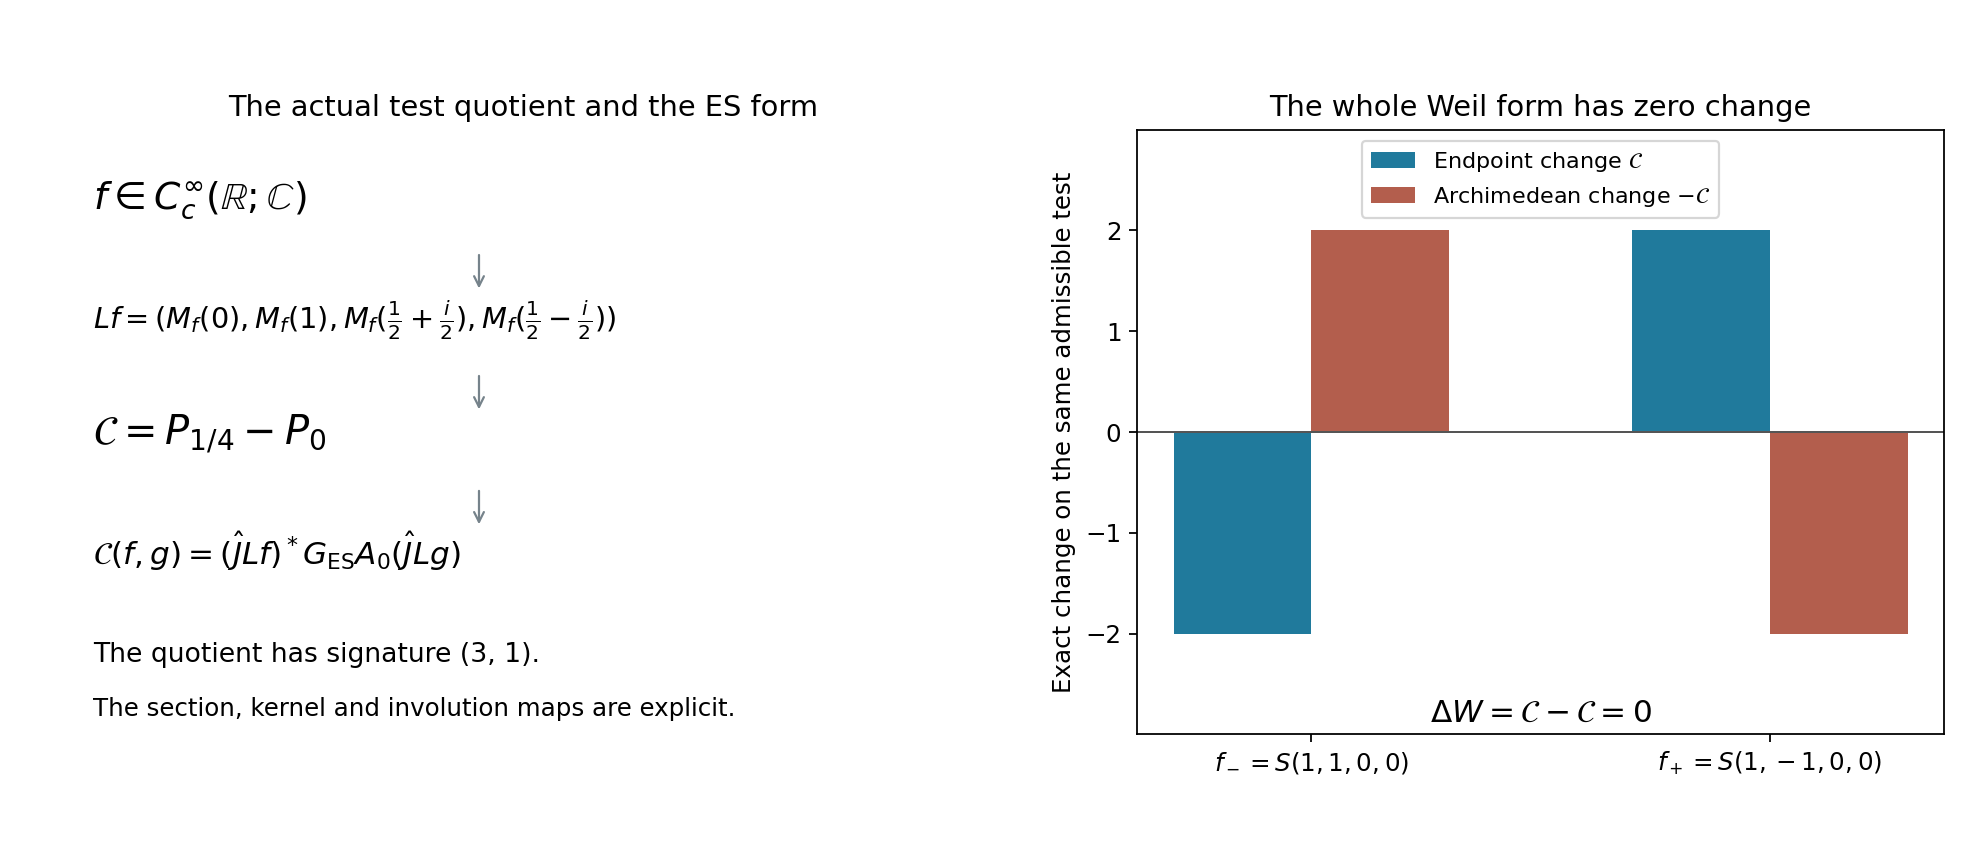
\includegraphics[keepaspectratio,alt={The actual four-value correction, its exact ES isometry, and its cancellation in the full Weil form. WEC1--WEC18 give all maps, the section and the two admissible tests.}]{figures/29_actual_weil_correction.png}}
\caption{The actual four-value correction, its exact ES isometry, and
its cancellation in the full Weil form. WEC1--WEC18 give all maps, the
section and the two admissible tests.}
\end{figure}

\end{document}
